\documentclass{article}
\usepackage{wrapfig}
\usepackage{graphicx}

\begin{document}
\begin{wrapfigure}{l}{25mm}
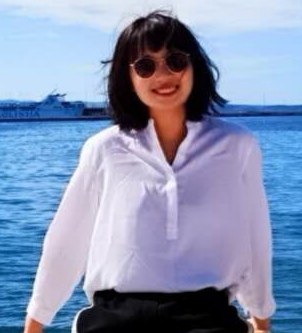
\includegraphics[width=1in,height=1.25in,clip,keepaspectratio]{author/profile.jpeg}
\end{wrapfigure}\par
\textbf{Hanwei Zhang} Hanwei Zhang is a Post-doctoral researcher on the QARMA team at LIS Marseille, working on the interpretability of deep neural networks with Ronan Sicre, Stephane Ayache, and Yannis Avrithis. She defended her Ph.D. thesis on "Deep Learning in Adversarial Context" in 2021, which focused on the security problem in machine learning and was supervised by Laurent Amsaleg, Yannis Avrithis, and Teddy Furon in the Linkmedia team at IRISA Rennes. Her current work primarily focuses on trustworthy AI, including interpretability and adversarial security of machine learning models.\par

\begin{wrapfigure}{l}{25mm}
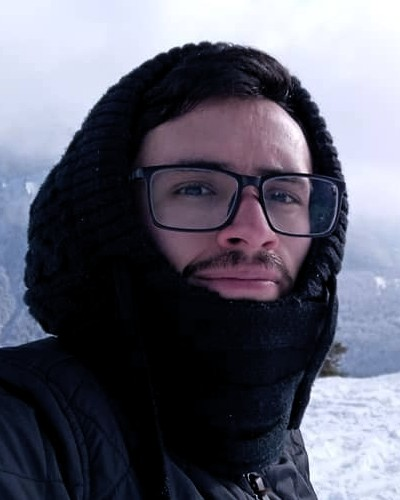
\includegraphics[width=1in,height=1.25in,clip,keepaspectratio]{author/felipe.jpg}
\end{wrapfigure}\par
\textbf{Felipe Torres} Felipe Torres is a Ph.D. student in Interpretable recognition at École Centrale Marseille, on the research team QARMA since October 2020, under supervision of Ronan Sicre, Stephane Ayache, and Yannis Avrithis. He is interested in Machine Learning and Computer Vision (CV), on new technologies or applications. From 2016 to 2020, he worked on Biomedical Images (namely bone age assessment) via classification/regression in the Biomedical Computer Vision Group at Universidad de los Andes, under the tutelage of professor Pablo Arbeláez. \par

\begin{wrapfigure}{l}{25mm}

\includegraphics[width=1in,height=1.25in,clip,keepaspectratio]{author/ronan.jpeg}
\end{wrapfigure}\par
\textbf{Ronan Sicre} Ronan Sicre received a Master degree in Intelligent Systems from the University of Toulouse, France, in 2007. During his master he studied at the University of Plymouth, England, at the University of Calgary, Canada, and at the Technical University of Berlin, Germany. From 2008 to 2011, he worked toward the Ph.D. degree in the LaBRI at the University of Bordeaux in collaboration with MIRANE S.A.S. Then, he obtained a Lecturer / Researcher (ATER) position in Bordeaux: he taught at the ENSEIRB-MATMECA and worked as a researcher at the LaBRI. he then worked as a postdoc at the University of Amsterdam (UvA) at the Intelligent System Lab (ISLA), at the University of Caen, in the image team of the GREYC lab, and at INRIA Rennes in the Linkmedia Team. He is now Assistant professor at Ecole Centrale Marseille and belong to the QARMA team at LIS \par

\begin{wrapfigure}{l}{25mm}
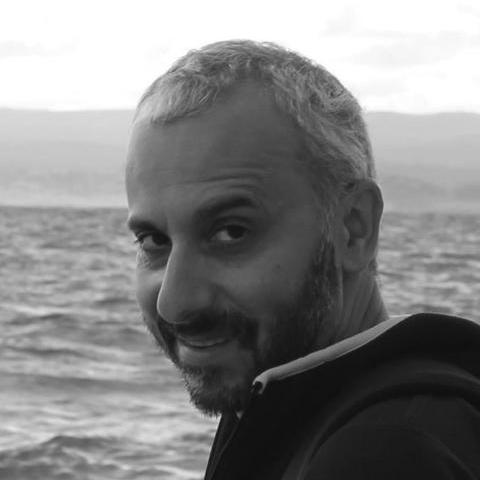
\includegraphics[width=1in,height=1.25in,clip,keepaspectratio]{author/iavr.jpg}
\end{wrapfigure}\par
\textbf{Yannis Avrithis} Since 2022 Yannis Avrthis is a Principal Investigator at the Institute of Advanced Research on Artificial Intelligence (IARAI), carrying out research on computer vision and machine learning. Between 2021 and 2022 he has been a Research Director at the Information Management Systems Institute (IMSI) of Athena Research Center. His recent work is focusing on different learning settings including metric learning, incremental learning, and few-shot learning; multimodal learning including vision, language, and 3D models; interpretability; and video question answering.
Between 2016 and 2021 he has been a research scientist in the LinkMedia team of Inria Rennes-Bretagne Atlantique and he has been teaching Deep Learning for Vision at the University of Rennes 1. His work has focused on exploring the manifold structure of data and, apart from image retrieval, using it for unsupervised, semi-supervised, and few-shot learning. He has also worked on adversarial examples and on investigating the sparsity of convolutional activations, applied to spatial matching and unsupervised object discovery. In 2020, he was awarded the Habilitation à Diriger des Recherches (HDR) qualification from the University of Rennes 1.\par

\begin{wrapfigure}{l}{25mm}
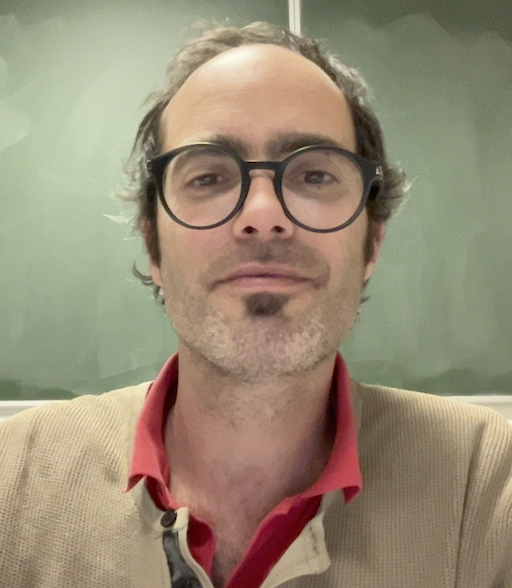
\includegraphics[width=1in,height=1.25in,clip,keepaspectratio]{author/SA.png}
\end{wrapfigure}\par
\textbf{Stephane Ayache}Stephane Ayache is assistant professor at Aix-Marseille University since 2008. His research areas are machine learning and computer vision with a special interest on multimodal representations and representation understanding. He co-organized challenges and workshops at ECML, CVPR, NIPS and published more than 70 papers.\par
\end{document}